\documentclass[a4paper,11pt]{scrartcl}%scrbook %[...,twoside]

\usepackage[a4paper,left=3.5cm,right=2.5cm,bottom=3.5cm,top=3cm]{geometry}

\usepackage[ngerman]{babel}

% Caption Packet
\usepackage[margin=0pt,font=small,labelfont=bf]{caption}
% Gliederung einstellen
%\setcounter{secnumdepth}{5}
%\setcounter{tocdepth}{5}
%\usepackage[Sonny]{fncychap}
%\ChTitleVar{\huge\rm}
\usepackage[pdftex]{graphicx,color}
\usepackage{amsmath,amssymb}
% Theorem-Umgebungen
\usepackage[amsmath,thmmarks]{ntheorem}
% Korrekte Darstellung der Umlaute
\usepackage[utf8]{inputenc}
\usepackage[T1]{fontenc}
\usepackage{lmodern}
\usepackage[onehalfspacing]{setspace}
% Algorithmen
\usepackage{algorithm}
\usepackage{algorithmic}
%\renewcommand{\algorithmiccomment}[1]{\hfill \tiny//~#1\normalsize}
% Bibtex deutsch
\usepackage{bibgerm}
% URLs
\usepackage{url}
\usepackage{verbatim}
\usepackage{algorithm}

% Theorem-Optionen %
\theoremseparator{}
\theoremstyle{change}
\newtheorem{theorem}{Theorem}[section]
\newtheorem{satz}[theorem]{Satz}
\newtheorem{lemma}[theorem]{Lemma}
\newtheorem{korollar}[theorem]{Korollar}
\newtheorem{proposition}[theorem]{Proposition}
% Ohne Numerierung
\theoremstyle{nonumberplain}
\renewtheorem{theorem*}{Theorem}
\renewtheorem{satz*}{Satz}
\renewtheorem{lemma*}{Lemma}
\renewtheorem{korollar*}{Korollar}
\renewtheorem{proposition*}{Proposition}
% Definitionen mit \upshape
\theorembodyfont{\upshape}
\theoremstyle{change}
\newtheorem{definition}[theorem]{Definition}
\theoremstyle{nonumberplain}
\renewtheorem{definition*}{Definition}
% Kursive Schrift
\theoremheaderfont{\itshape}
\newtheorem{notation}{Notation}
\newtheorem{konvention}{Konvention}
\newtheorem{bezeichnung}{Bezeichnung}
\theoremsymbol{\ensuremath{\Box}}
\newtheorem{beweis}{Beweis}
\theoremsymbol{}
\theoremstyle{change}
\theoremheaderfont{\bfseries}
\newtheorem{bemerkung}[theorem]{Bemerkung}
\newtheorem{beobachtung}[theorem]{Beobachtung}
\newtheorem{beispiel}[theorem]{Beispiel}
\newtheorem{problem}{Problem}
\theoremstyle{nonumberplain}
\renewtheorem{bemerkung*}{Bemerkung}
\renewtheorem{beispiel*}{Beispiel}
\renewtheorem{problem*}{Problem}
%
%% Algorithmen anpassen %
%\renewcommand{\algorithmicrequire}{\textit{Eingabe:}}
%\renewcommand{\algorithmicensure}{\textit{Ausgabe:}}
%\floatname{algorithm}{Algorithmus}
%\renewcommand{\listalgorithmname}{Algorithmenverzeichnis}
%\renewcommand{\algorithmiccomment}[1]{\color{grau}{// #1}}
%
% Floating-Umgebungen anpassen %
\renewcommand{\topfraction}{0.9}
\renewcommand{\bottomfraction}{0.8}
% Abkuerzungen richtig formatieren %
\usepackage{xspace}
\newcommand{\vgl}{vgl.\@\xspace} 
\newcommand{\zB}{z.\nolinebreak[4]\hspace{0.125em}\nolinebreak[4]B.\@\xspace}
\newcommand{\bzw}{bzw.\@\xspace}
\newcommand{\dahe}{d.\nolinebreak[4]\hspace{0.125em}h.\nolinebreak[4]\@\xspace}
\newcommand{\etc}{etc.\@\xspace}
\newcommand{\evtl}{evtl.\@\xspace}
\newcommand{\ggf}{ggf.\@\xspace}
\newcommand{\bzgl}{bzgl.\@\xspace}
\newcommand{\so}{s.\nolinebreak[4]\hspace{0.125em}\nolinebreak[4]o.\@\xspace}
\newcommand{\iA}{i.\nolinebreak[4]\hspace{0.125em}\nolinebreak[4]A.\@\xspace}
\newcommand{\sa}{s.\nolinebreak[4]\hspace{0.125em}\nolinebreak[4]a.\@\xspace}
\newcommand{\su}{s.\nolinebreak[4]\hspace{0.125em}\nolinebreak[4]u.\@\xspace}
\newcommand{\ua}{u.\nolinebreak[4]\hspace{0.125em}\nolinebreak[4]a.\@\xspace}
\newcommand{\og}{o.\nolinebreak[4]\hspace{0.125em}\nolinebreak[4]g.\@\xspace}
\newcommand{\oBdA}{o.\nolinebreak[4]\hspace{0.125em}\nolinebreak[4]B.\nolinebreak[4]\hspace{0.125em}d.\nolinebreak[4]\hspace{0.125em}A.\@\xspace}
\newcommand{\OBdA}{O.\nolinebreak[4]\hspace{0.125em}\nolinebreak[4]B.\nolinebreak[4]\hspace{0.125em}d.\nolinebreak[4]\hspace{0.125em}A.\@\xspace}

% Leere Seite ohne Seitennummer, naechste Seite rechts
\newcommand{\blankpage}{
 \clearpage{\pagestyle{empty}\cleardoublepage}
}
\bibliographystyle{unsrt}
\usepackage{hyperref}
% Keine einzelnen Zeilen beim Anfang eines Abschnitts (Schusterjungen)
\clubpenalty = 10000
% Keine einzelnen Zeilen am Ende eines Abschnitts (Hurenkinder)
\widowpenalty = 10000 \displaywidowpenalty = 10000
% EOF
\titlehead{
	\begin{minipage}{7.2cm}
		\vspace{-6mm}
		\hspace{-4mm}
	\includegraphics[scale=0.5]{./logo}
	\end{minipage}
	\begin{minipage}{7.6cm}
		\begin{flushright}
			Fakultät für Informatik\\
			Lehrstuhl für Algorithm Engineering (LS11)\\
			http://ls11-www.cs.tu-dortmund.de\\
		\end{flushright}
  \end{minipage}
  \\
	\centerline{\hrulefill}
}%end of titlehead


\title{\vspace{2,5cm}Textkompression mithilfe einer Variante von LZ78}
\subtitle{Exposee}
\author{Florian Kleine\\Matrikelnummer: 157020}
\publishers{\parbox[b][12cm]{\textwidth}{Betreuer:\\ Prof. Dr. Johannes Fischer\\
Dominik Köppl}}
\date{\today}



\begin{document}
\maketitle
\thispagestyle{empty}
\newpage
\tableofcontents
\newpage
\newpage
\section{Einleitung}

Die Datenkompression spielt in der Informatik eine große Rolle. Zwar sind die Datenträger im Vergleich zu früher um ein Vielfaches größer und vor allem günstiger geworden, stoßen bei den heute anfallenden riesigen Datenmengen aber immer noch an ihre Grenzen. Deshalb ist es sinnvoll die Daten mit geschickten Verfahren so zu komprimieren, dass sie später verlustfrei in den Ursprungszustand zurückübersetzt werden können.
In dieser Arbeit soll es darum gehen, Texte mithilfe einer Variante des Lempel-Ziv78-Verfahrens in Faktoren zu zerlegen, zu kodieren und so verlustfrei zu komprimieren. Dieses Verfahren stützt sich auf der Eliminierung von Redundanzen, indem Teile des Textes durch Verweise auf vorher auftretende gleiche Teile ersetzt werden. Solche Verweise benötigen weniger Speicher als der Text, was so zu einer Kompression des kompletten Textes führt.
Das aus dieser Arbeit entstehende Verfahren wird anschließend mit bereits vorhandenen Kompressionsverfahren (z.B. gzip und 7zip) verglichen.\\\\

\section{Entwurf einer Gliederung}

	\begin{itemize}
		\item Einleitung
		\item Theoretische Grundlagen
		\item Entworfene Algorithmen
		\item Implementierung
		\item Praktische Tests
		\item Fazit
	\end{itemize}
\newpage	
\section{Leseprobe}
	\subsection{Theoretische Grundlagen}
	
	Im Folgenden werden Datenstrukturen und Operationen eingeführt, die in dieser Arbeit benötigt werden.\\
	Sei das Alphabet $\Sigma$ definiert als eine Menge von Zeichen, dann bezeichnet $\Sigma^{*}$ die Menge aller Worte, die aus dem Alphabet gebildet werden können. Jedes dieser Worte bezeichnet man als String.
	Sei $s$ ein String mit der Länge $n$.
	
	\begin{definition}[Länge]
		Sei $|s|$ die Länge des String $s$, das heißt die Anzahl von Zeichen in $s$.
	\end{definition}
	
	\begin{definition}[Leerstring]
		Sei $\varepsilon \in \Sigma$* der leere String. Es gilt $|\varepsilon|$ = 0.
	\end{definition}
	
	\begin{definition}[Symbolzugriff]
		Für $x \in \mathbb{N}$ und $x \leq n$ sei $s[x]$ das $x$-te Zeichen aus $s$.
	\end{definition}
	
	\begin{definition}[Teilstring]
		Für $x,y \in \mathbb{N}$ und $1 \leq x < y \leq n$ sei $s[x,y]$ die Zeichenfolge vom $x$-ten bis zum $y$-ten Zeichen aus $s$. $s$[x] und $s$[y] einschließlich.
	\end{definition}
	
	\begin{definition}[Suffix]
		 Für $x \in \mathbb{N}$ und $x \leq n$ sei $s[x..]$ das $x$-te Suffix von $s$. Also gilt $s[x..] = s[x,n]$.
	\end{definition}
	
	\begin{definition}[Suffix-Tree]
		Ein Suffix-Tree eines Strings $s$ ist ein Baum mit $n$ Blättern. Alle inneren Knoten erfüllen folgende Bedingungen:
		\begin{itemize}
			\item Jeder Knoten hat mindestens 2 Kinder.
			\item Jede Kante ist mit einem nicht-leeren Teilstring von $s$ markiert.
			\item Die Markierung ausgehender Kanten eines Knotens beginnen nicht mit dem gleichen Zeichen.
			\item Die Konkatenation von allen Zeichen auf dem Pfad von der Wurzel zum Blatt $i$ ist das $i$-te Suffix $s[i..]$ von $s$.
		\end{itemize}
		\begin{beispiel}[Suffix-Tree]
			$s$ = \texttt{ananas\$}
			\begin{figure}
				\centering
				  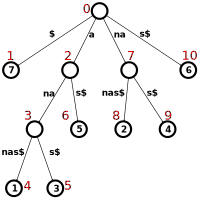
\includegraphics[scale=0.8]{./pics/ananas_suffixTree_inorder}
				  \cite{suffixtreeurl}
				  \caption{Diese Abbildung zeigt den Suffix-Tree zu $s$ = \texttt{ananas\$}. Die Blätter sind hierbei nummeriert. Der String auf dem Pfad von der Wurzel zum Blatt $i$ repräsentiert das Suffix $s[i..]$. Die roten Zahlen an den Knoten sind durch eine Pre-Order-Nummerierung entstanden und sind die IDs der Knoten. }
				  \label{fig:suffixTree}
			\end{figure}
		\end{beispiel}
		
	\end{definition}
	\newpage
	\subsection{Idee der LZ78 Variante}
	\subsubsection{LZ78}
	LZ78 wurde 1978 von Jacob Ziv und Abraham Lempel erfunden und ist ein Verfahren zur Datenkompression. Der (naive) Algorithmus durchläuft den String bzw. den Text $T$ und ersetzt Redundanzen durch Verweise auf das längste vorherige Vorkommen des selben Teils und hängt das nächste Zeichen an diesen Verweis an. Dadurch wird ein Baum erzeugt, der sog. LZ78-Trie. Dieses Verfahren wird nun am Beispiel von $T$ = \texttt{ananas\$} verdeutlicht.
	\begin{figure}[h]
	\begin{tabular}[t]{cc}
		\begin{tabular}[b]{l c c c c c}\hline
			& 1 & 2 & 3 & 4 & 5 \\ \hline
		   Textteil & \texttt{a} & \texttt{n} & \texttt{an} & \texttt{as} & \texttt{\$}\\ \hline
		   Faktorzerlegung & (-,\texttt{a}) & (-,\texttt{n}) & (1,\texttt{n}) & (1,\texttt{s}) &  (-,\texttt{\$})\\ \hline
		\end{tabular} & 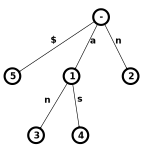
\includegraphics{./pics/ananas_LZ78Tree}
	\end{tabular}
	\caption{Links sieht man die Faktorisierung nach LZ78 und rechts den entsprechenden LZ78-Tree. Der $i$-te Faktor $(x,s)$ wird zu einem neuen Knoten $i$ mit $x$ als Elternknoten und die Kante $(x,i)$ wird mit $s$ beschriftet.}
	\label{fig:lz78}
	\end{figure}
	
	Ein \textit{Faktor} ist ein Tupel $(x,s)$ mit $x \in \{1..z\} \cup \{-\}$ und $s \in \Sigma$. $x$ bezeichnet hierbei den Elternknoten im LZ78-Tree und $s$ die Kantenbeschriftung der Kante von $x$ zum neu entstehenden Knoten. $z$ ist die Anzahl der Faktoren. Die Zahlen in den Knoten stehen für die Faktoren. 
	
	\subsubsection{LZ78 Variante}\label{sec:lz78-variante}
	Im Gegensatz zu LZ78 kann diese Variante (im Folgenden LZ78V genannt) auch mehr Zeichen an eine Ersetzung anhängen.
	Im Beispieltext $T$ = \texttt{ananas\$} folgt nach einem \texttt{'n'} immer ein \texttt{'a'}. Dies spiegelt sich im Suffix-Tree durch die Kantenbeschriftung \texttt{'na'} wider. Mit LZ78V können wir nun beim ersten Lesen von \texttt{'n'} den Faktor (-,\texttt{na}) erstellen, denn nach \texttt{'n'} kann nichts anderes kommen. Es ergibt sich folgende Faktorzerlegung:\\
	\begin{figure}[h]
	\begin{tabular}[t]{c c c}
		\begin{tabular}[b]{l c c c}\hline
			& 1 & 2 & 3  \\ \hline
  		Textteil & \texttt{a} & \texttt{na} & \texttt{nas\$} \\ \hline
  		Faktorzerlegung & (-,\texttt{a}) & (-,\texttt{na}) & (2,\texttt{s\$}) \\ \hline
		\end{tabular} & \hspace{2cm} & 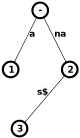
\includegraphics{./pics/ananas_LZ78VTree}\\\\
	\end{tabular}
	\caption{Links sieht man die Faktorisierung nach LZ78V und rechts den entsprechenden LZ78V-Tree. Der $i$-te Faktor $(x,s)$ wird zu einem neuen Knoten $i$ mit $x$ als Elternknoten und die Kante $(x,i)$ wird mit $s$ beschriftet. Im Gegensatz zum LZ78-Tree kann $s$ aber mehr als ein Zeichen beinhalten.}
	\label{fig:lz78v}
	\end{figure}
	
	Den LZ78V-Tree können wir mit einem zweidimensionalen Array $A$ repräsentieren. So wäre $A[i][1] = x$ und $A[i][2] = s$ der $i$-te Faktor $(x,s)$ in der Array-Darstellung. Im Beispiel $T$ = \texttt{ananas\$} ergibt sich:\\\\
	\begin{tabular}[b]{l c c c}
						\hline
							& 1 & 2 & 3 \\\hline
						$A[1]$ & - & - & 2 \\\hline
						$A[2]$	& \texttt{a} & \texttt{na} & \texttt{s\$}\\\hline
						
			
	\end{tabular}
	
	
	
	
	
	
	Gehen wir jedoch strikt nach diesem Verfahren vor, kann es aber auch zu einer schlechteren Faktorisierung kommen. Schlecht definieren wir hier über die Gesamtanzahl der Buchstaben in der Faktorisierung. Je mehr Buchstaben, desto schlechter ist die Faktorisierung.  Beispielweise beim Text $T$ = \texttt{abrakabrabra\$} würde LZ78V den Text in 3 Faktoren zerlegen: (-,\texttt{a})(-,\texttt{bra})(-,\texttt{kabrabra}) mit insgesamt 12 Buchstaben.\\
	Dies entsteht dadurch, dass sobald man ein \texttt{'k'} liest, die restlichen Zeichen eindeutig durch den Suffix-Tree bestimmt werden können und somit zu einem Faktor zusammengefasst werden. In dieser Arbeit soll hierfür eine Lösung gefunden werden. Es wäre zum Beispiel denkbar, $(x,s)$ mit $x \in \{1...z\} \cup \{-\}$ und $s \in \Sigma^{+}$ nur in die Faktorisierung aufzunehmen, wenn der entsprechende Knoten im Suffix-Tree mindestens 2 Kinder hat. Ansonsten nehmen wir nur das erste Zeichen von $s$.\\ Am Beispiel $T$ = \texttt{abrakabrabra\$} ergibt sich dann:\\
	(-,\texttt{a})(-,\texttt{bra})(-,\texttt{k})(1,\texttt{bra})(2,\texttt{\$}) mit insgesamt 9 Buchstaben.

	
	\subsection{Idee des Algorithmus}
	
		\begin{algorithm}[H]
		\begin{algorithmic}
			\STATE ST = constructST($T$) \COMMENT{mithilfe von \textit{sdsl}}
			\STATE x = ST.size()
			\STATE U = bit\_vector(x, 0) \COMMENT{Bitvektor mit x Einträgen, mit 0 initialisiert}
			\STATE F = int\_vector(0, 0, $\lfloor \log x\rfloor$ + 1) \COMMENT{leerer Vektor mit $\lfloor \log x\rfloor$ + 1 Bits für jeden Eintrag}
			\STATE U[ST.root().id()] = 1 \COMMENT{markiere die Wurzel als benutzt}
			\STATE current\_node = ST.root() \COMMENT{Startknoten ist die Wurzel von ST}
			\STATE t = 0
			\WHILE {not current\_node.is\_leaf()}
				\STATE current\_node = ST.nextNode(current\_node, T[t]) \COMMENT{nächsten Knoten in ST finden}
				\STATE t = t + ST.string\_on\_edge(current\_node).length() \COMMENT{Textposition entsprechend verändern}
				\IF {U[current\_node.id()] == 1} 
					\STATE continue \COMMENT{suche mit dem nächsten Zeichen den nächsten Knoten}
				\ELSE
					\STATE F.add(current\_node.id()) \COMMENT{ID des aktuellen Knotens an $F$ anhängen}
					\STATE U[current\_node] = 1 \COMMENT{aktuellen Knoten als benutzt markieren}
					\STATE current\_node = ST.root() \COMMENT{beginne im nächsten Durchlauf wieder an der Wurzel}
				\ENDIF
			\ENDWHILE
		
			
		\end{algorithmic}	
		\caption{Faktorisierung von Text $T$ nach LZ78V mit Vektoren}
		\label{algoLZ78V1}
		\end{algorithm}
		
		Um einen Text $T$, wie in Kapitel \ref{sec:lz78-variante} in Faktoren zu zerlegen, konstruieren wir uns zuerst den Suffix-Tree $ST$. Hierzu wird die C++ Bibliothek \textit{sdsl} verwendet. Mit Hilfe dieser Bibliothek lassen sich sog. \textit{Compressed Suffix Trees} (CST) leicht aus Texten erzeugen. Außerdem besitzt jeder Knoten in $ST$ eine eindeutige ID aus dem Bereich 0 bis $x-1$, wenn $x$ die Anzahl der Knoten in $ST$ ist. Nachdem wir $ST$ erstellt haben, erzeugen wir wieder mit Hilfe von \textit{sdsl} einen Bit-Vektor $U$ mit $x$ Einträgen und initialisieren ihn mit 0. Der Vektor $U$ speichert für jeden Knoten $v$ mit der ID $i$, ob er schon als Faktor benutzt wird. Falls dieser Knoten $v$ bereits als Faktor benutzt wird, ist U[$i$] = 1. Wir setzen U[id(root())] = 1, da die Wurzel nie als Faktor verwendet wird. Außerdem erzeugen wir mit Hilfe von \textit{sdsl} einen sog. \textit{int\_vector} $F$, der für jeden Eintrag $\lfloor\log x\rfloor + 1$ Bits belegt.
		Nun beginnen wir den Text zu lesen. Der aktuelle Knoten $current\_node$ in $ST$ ist die Wurzel. Anhand des ersten Zeichens von $T$ können wir bestimmen, welche Kante man nehmen muss und aktualisieren $current\_node$ mit dem entsprechenden Knoten. Außerdem setzen wir die aktuelle Textposition $t$ um so viele Zeichen weiter wie an der Kante zu $current\_node$ stehen. Wir testen, ob $current\_node$ schon als Faktor benutzt wird. Das heißt wir testen, ob U[$current\_node$] = 1 ist. Wenn ja, suchen wir uns anhand des nächsten Zeichens in $T$ den nächsten Knoten in $ST$ und verfahren mit diesem Knoten analog.
		Wenn nein, setzen wir $U[current\_node.id()] = 1$ und hängen $current\_node.id()$ an $F$ an. Dann beginnen wir mit dem nächsten Zeichen von $T$ an der Wurzel von $ST$ erneut. Dies wiederholen wir solange, bis der $current\_node$ ein Blatt von $ST$ ist. Dann können wir die Faktorisierung beenden, da der Text zu Ende ist.
		\begin{figure}[h]
			\centering
			\includegraphics[scale=0.8]{./pics/ananas_suffixTree_inorder_markiert}
			\caption{Die blauen, dicken Kreise visualisieren die Knoten, die wir in $F$ als Faktoren benutzen. Sonstige Nummerierungen entsprechen den Angaben aus Abbildung \ref{fig:suffixTree}.}
			\label{fig:st_inorder}
		\end{figure}
		\\Im Beispiel von $T$ = \texttt{ananas\$} und den IDs aus Abbildung \ref{fig:st_inorder}  ergibt sich: \\
		$U$ = [1,0,1,0,0,0,0,1,0,1,0] und $F$ = [2,7,9].\\
		
		Der beschriebene Algorithmus hat lineare Laufzeit. Im Folgenden sei $n$ die Länge des Textes $T$, $x$ die Anzahl der Knoten in $ST$ und $y$ die Anzahl der Faktoren in $F$.
		Der Speicherbedarf zur Laufzeit beträgt 3$n$ + o($n$) + $\arrowvert$CSA$\arrowvert$ + $\arrowvert$LCP$\arrowvert$ Bits für $ST$\cite{cheetsheet}, $x$ Bits für den Bit-Vektor $U$ und $y * (\lfloor\log(x)\rfloor+1)$ Bits für $F$. \\Also insgesamt 3$n$ + o($n$) + $\arrowvert$CSA$\arrowvert$ + $\arrowvert$LCP$\arrowvert$ + $x$ + $y$ * $\lfloor\log$ $x\rfloor$ + $y$ Bits.\\
		Um die Tabelle $A$ nun mit Faktoren zu füllen, erstellen wir uns mit \textit{sdsl} einen int\_vector $N$ mit $z$ Einträgen. Jeder Eintrag belegt $\lfloor \log z\rfloor + 1$ Bits, also insgesamt belegt der \\Vektor $N$ $z * \lfloor \log z\rfloor + z$ Bits. Dieser Vektor soll für jede ID aus $F$ speichern, den wievielten Faktor der entsprechende Knoten repräsentiert. Mithilfe von $sdsl$ bauen wir auf $U$ eine $rank$ - Struktur auf. Diese hilft uns $N$ zu füllen. Dafür laufen wir $F$ einmal von links nach rechts durch und setzen $N[U.rank[F[j]]] = j$ für jeden Eintrag in $F$ an der Position $j$. Im Beispiel von $T$ = \texttt{ananas\$} ist $N = [1,2,3]$.
		Den Speicher von $F$ können wir jetzt freigeben. Nun lässt sich mithilfe von $U$, $N$ und $ST$ die Tabelle $A$ in linearer Zeit füllen. Dazu laufen wir $U$ einmal von links nach rechts durch und erstellen für jeden Eintrag in $U$ mit dem Index $i$, der ungleich 0 ist, einen Faktor in $A$ an der Stelle $N[U.rank[i]]$. Ist der Vaterknoten $p$ des entsprechenden Knoten in $ST$ die Wurzel verweist der Faktor auf 0. Ansonsten auf $N[U.rank[p.id()]]$. Außerdem enthält der Faktor den Text, der an der Kante zu diesem Knoten steht.
		\begin{algorithm}[H]
		\begin{algorithmic}
			\STATE ST = constructST($T$) \COMMENT{mithilfe von \textit{sdsl}}
			\STATE B.root = node(0, ST.root().id())
			\STATE ST\_current\_node = ST.root()
			\STATE B\_current\_node = B.root()
			\STATE t = 0, k = 0 \COMMENT{t ist die aktelle Textposition, k die aktuelle Anzahl der Faktoren}
			\WHILE {not ST\_current\_node.isLeaf()}
				\STATE ST\_current\_node = ST.nextNode(ST\_current\_node, T[t]) \COMMENT{nächster Knoten in ST}
				\IF {B\_current\_node.dict.exist(T[t])}
					\STATE B\_current\_node = B\_current\_node.dict.find(T[t]) \COMMENT{gehe gleichen Pfad wie in ST}
					\STATE t = t + ST.string\_on\_edge(ST\_current\_node, T[t]) + 1
					\STATE continue
				\ELSE
					\STATE new\_node = node(k, ST\_current\_node.id()) \COMMENT{es muss ein Knoten eingefügt werden}
					\STATE B\_current\_node.dict.insert(T[t], *new\_node)
					\STATE t = t + ST.string\_on\_edge(ST\_current\_node, T[t]) + 1 
					\STATE B\_current\_node = B.root() \COMMENT{beginne wieder an beiden Wuzeln mit dem nächsten Zeichen}
					\STATE ST\_current\_node = ST.root()
					\STATE k = k + 1
				\ENDIF 
			\ENDWHILE
		
		\end{algorithmic}	
		\caption{Faktorisierung von Text $T$ nach LZ78V mit Baumstruktur}
		\label{algoLZ78V2}
		\end{algorithm}
		
		Eine Alternative zu Algorithmus \ref{algoLZ78V1} ist, dass wir während der Faktorisierung den LZ78V-Tree aufbauen. Hierzu erstellen wir einen Baum $B$, der nur die Wurzel als Knoten enthält. Ein Knoten repräsentiert ein Tupel ($a ,b$), wobei $a$ die ID des Knotens ist und angibt, als wievielter dieser Knoten hinzugefügt wurde. $b$ ist die ID des entsprechenden Knotens in $ST$. Außerdem enthält jeder Knoten ein dynamisches Dictionary, das Zeichen mit Pointern verknüpft. Diese Pointer zeigen auf die Kindknoten eines Knotens. Das Dictionary benötigt $s_{dict}$($m$) zum Speichern von $m$ Elementen. Die Laufzeit eines Look-Ups beträgt $t_{lookup}$($m$) und das Einfügen $t_{insert}$($m$). Während wir, wie in Algorithmus \ref{algoLZ78V1} beschrieben, anhand der gelesenen Zeichen $ST$ durchlaufen, versuchen wir den gleichen Pfad auch in $B$ zu gehen. Kommen wir an den Punkt, wo dies in $B$ nicht möglich ist, erstellen wir den entsprechenden Knoten in $B$ und beginnen in beiden Bäumen mit dem nächsten Zeichen von vorn. Sind wir in $ST$ an einem Blattknoten angelangt, kann man die Faktorisierung beenden, da der Text zu Ende ist. So ergibt sich im Beispiel $T$ = \texttt{ananas\$} der Baum aus Abbildung \ref{fig:ausschnitt}. 
			\begin{figure}[h]
				\centering
				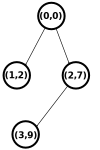
\includegraphics[scale=0.8]{./pics/ananas_LZ78VTree(ausschnitt)}
				\caption{Dies ist der Baum $B$ zu $T$ = \texttt{ananas\$} nach der Faktorisierung unter Berücksichtigung der IDs aus Abbildung \ref{fig:st_inorder}.}
				\label{fig:ausschnitt}
			\end{figure}
		Diese Alternative ist besonders gut, wenn die Anzahl $z$ der Faktoren klein ist. Denn der Speicherbedarf des Baums beträgt $z * (\lfloor\log x\rfloor + \lfloor\log z\rfloor + 2)$ + $\sum_{k=1}^z s_{dict}^{(k)}$ Bits und die Laufzeit ist $O(n * t_{lookup}(z)$). Hinzu kommt noch der Speicherbedarf von $ST$.
		Mit $B$ und $ST$ können wir auch in linearer Zeit die Tabelle $A$ füllen. Wir durchlaufen den Baum z.B. in Pre-Order. Für jeden Knoten, außer der Wurzel,  erstellen wir in $A$ an der Position $a$ einen Faktor. Dieser verweist auf die ID des Elternknotens in $B$ und enthält den Text, der in $ST$ an der Kante zum Knoten mit der ID $b$ steht.
		
		
		
	
	
	
	
	\subsection{Mögliche Kodierung}
	
	Eine Möglichkeit die Tabelle $A$ zu kodieren wäre die Huffman Kodierung. Diese Kodierung ordnet jedem Symbol einen präfixfreien Code zu. Dazu ordnen wir die Symbole nach der Häufigkeit ihres Auftretens und erstellen für jedes Symbol einen Knoten, der die Häufigkeit des Auftretens enthält. Nun fügen wir zwei Knoten (bzw. Teilbäume) mit kleinster Häufigkeit zu einem neuen Teilbaum zusammen. Die Wurzel enthält dabei die Summe der beiden Häufigkeiten der Teilbäume. Dies wiederholen wir solange, bis nur noch ein Baum übrig ist. Für jedes Symbol können wir nun auf dem Pfad von der Wurzel zum Blattknoten(Blätter enthalten die Symbole) einen Code ablesen: 0 für das linke Kind und 1 für das rechte Kind. \\
	In der Kodierung der Tabelle $A$ müssen wir noch zwischen Verweisen und Zeichen des Textes unterscheiden. Daher markieren wir die Verweise mit einen *. So ergibt sich beim Beispiel $T = \texttt{ananas\$}$ der zu kodierende Text: \texttt{$0^*a0^*na2^*s\$$}.
	\begin{figure}[h]
			\centering
			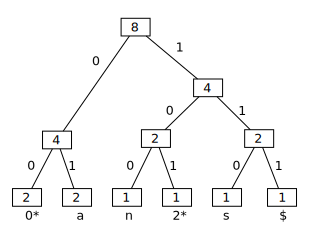
\includegraphics[scale=0.8]{./pics/huffmanTree}
			\caption{Diese Abbildung zeigt einen möglichen Huffman-Tree zum Text \texttt{$0^*a0^*na2^*s\$$}. Der Code für jedes Symbol ist der String auf dem Pfad bis zum Blatt des Symbols.}
			\label{fig:huffman}
	\end{figure}
	\\Mit dem Huffman-Tree aus Abbildung \ref{fig:huffman}  ergibt sich folgende Kodierung für $T$ = \texttt{ananas\$}:
	00010010001101110111.
	Diese Art der Kodierung hat den Vorteil, dass Symbole, die häufig vorkommen, einen kürzeren Code bekommen als Symbole mit niedriger Häufigkeit.
	\\Um den Huffman-Tree abzuspeichern, starten wir bei der Wurzel und gehen wie folgt vor:
	\begin{itemize}
		\item bei einem Knoten speichere 1 und das Zeichen am Blatt
		\item sonst speichere 0 und verfahre mit den Kindknoten auf die gleiche Weise (erst links, dann rechts)
	\end{itemize}
	
	So ergibt sich für den Huffman-Tree aus dem Beispiel: $0010^*1a001n12^*01s1\$$
	\section{Ziele der Arbeit}
	
	In dieser Arbeit soll eine Variante des LZ78-Verfahrens entwickelt und in C++, unter der Verwendung der C++ Bibliothek \textit{sdsl}, implementiert werden. Dieses soll Texte und Dateien besser komprimieren als LZ78. Außerdem soll ein gutes Verfahren gefunden oder selbst entwickelt werden, um die Faktorisierung nach dieser LZ78-Variante zu kodieren. Denn nur so lässt sich diese Kompression mit Kompressionen anderer Verfahren, wie z.B. gzip oder 7zip, vergleichen. Kriterien für den Vergleich sind die relative Anzahl von Bits der Ausgabe und die Geschwindigkeit beim Komprimieren bzw. Dekomprimieren. Testdaten entnehme ich hierbei aus \cite{textcollection}. Enthalten sind Source-Code in C und Java, Proteinsequenzen, DNA, englische Texte und XML-Dateien mit verschiedenen Alphabetgrößen. 
	\newpage
	\section{Zeitplan}
	\textbf{\underline{Meilensteine:}}
	\begin{itemize}
		\item bis April: \begin{itemize}
		\item Theoretische Grundlagen zu großen Teilen fertig (bei Bedarf später ergänzen)
		\item Programmbibliotheken festlegen
		\end{itemize}
			\item Mitte April: Algorithmus implementiert
			\item ab Mai: 
		\begin{itemize}
			\item Optimierung von Speicherbedarf und Geschwindigkeit
			\item Mit anderen Kompressionsverfahren vergleichen und Ergebnisse dokumentieren
		\end{itemize}
	\end{itemize}	
	Außerdem finden nach Absprache alle 2 Wochen Treffen mit dem Betreuer statt um eventuell auftretende Fragen zu klären und den aktuellen Stand der Abschlussarbeit sicherzustellen.
	
	
	
	\newpage
	\nocite{*}
	\bibliography{bibs}

	
	

\end{document}